\documentclass[dvipsnames]{article}
\usepackage[utf8]{inputenc}
\usepackage[english]{babel}
\usepackage{geometry}
\usepackage[T1]{fontenc}
\usepackage{graphicx}
\graphicspath{ {../Figures/} }
\setlength\parindent{0pt}
\usepackage{hyperref}
\hypersetup{colorlinks=true,linkcolor=blue,filecolor=magenta,urlcolor=cyan,}
\urlstyle{same}
\usepackage{amsthm}
\usepackage{amsmath}
\theoremstyle{definition}
\usepackage{pgfplots}
\usepackage{caption}
\usepackage{subcaption}
\usepackage{makecell}
\usepackage[table]{colortbl}
\usepackage{enumitem}
\usepackage{siunitx}
\usepackage{amssymb}
\usepackage{tikz-cd}
\tikzset{>=latex}
\usepackage{tkz-euclide}
\usepackage{tikz,bm}
\usepackage{mwe,tikz}
\usetikzlibrary{arrows}
\pgfplotsset{compat=1.11}
\usepackage{moresize}
\usepackage{bohr}
\usetikzlibrary{patterns}
\usepackage{wrapfig}
\usepackage{mdframed}
\usepackage{dashrule}
\usepackage{tikzsymbols}
\usepackage{fontawesome}
\usepackage{linearb} %for \BPwheel symbol in Unit 6
\usepackage{multicol}
\usepackage{glossaries}
\usepackage{cancel}
% \usepackage{circuitikz}
\sisetup{group-separator = {,}}
\usepgfplotslibrary{fillbetween}
\usetikzlibrary{math}
\numberwithin{equation}{section}
\numberwithin{figure}{section}




\DeclareSIUnit{\nothing}{\relax}
\def\mymu{\SI{}{\micro\nothing} }

\newtheorem{example}{Example}[section]
\newtheorem{exercise}{}[section]
\newtheorem{regla}{Rule}


\newcommand{\Solution}{{\footnotesize \color{cyan} SOLUTION }}


\def\endsolution{{\footnotesize \color{cyan} \hfill END OF SOLUTION }}

\newcommand{\cyanhrule}{{\color{cyan} \hrule }}

\def\redplus{\mathbin{\color{red} +}}
\def\redminus{\mathbin{\color{red} -}}
\def\redtimes{\mathbin{\color{red} \times}}


\def\openstax{https://openstax.org/books/physics/pages/1-introduction}
\def\openstaxfooter{\fancyfoot[C]{Access for free at \href{\openstax}{\openstax} \hfill \thepage}}


% The following needs to be added to each individual main.tex file so it doesn't interfere with exam headers:

%\usepackage{fancyhdr}
% \pagestyle{fancy}
% \renewcommand{\headrulewidth}{0pt}
% \renewcommand{\headruleskip}{0mm}
% \fancyhead{}
% \def\openstax{https://openstax.org/books/physics/pages/1-introduction}
% \def\openstaxfooter{\fancyfoot[C]{Access for free at \href{\openstax}{\openstax} \hfill \thepage}}

\newcommand\myboxa[2][]{\tikz[overlay]\node[fill=gray!20,inner sep=4pt, anchor=text, rectangle, rounded corners=1mm,#1] {#2};\phantom{#2}}
\newcommand{\hgraydashline}{{\color{lightgray} \hdashrule{0.99\textwidth}{1pt}{0.8mm}}}

\let\oldtexttt\texttt% Store \texttt
\renewcommand{\texttt}[2][black]{\textcolor{#1}{\ttfamily #2}}% 

\newcommand\mybox[2][]{\tikz[overlay]\node[fill=black!20,inner sep=2pt, anchor=text, rectangle, rounded corners=1mm,#1] {#2};\phantom{#2}}

\setlength{\columnsep}{1cm}
\setlength{\columnseprule}{1pt}
\def\columnseprulecolor{\color{cyan}}

\pgfdeclarehorizontalshading{visiblelight}{50bp}{
color(0.00000000000000bp)=(red);
color(8.33333333333333bp)=(orange);
color(16.66666666666670bp)=(yellow);
color(25.00000000000000bp)=(green);
color(33.33333333333330bp)=(cyan);
color(41.66666666666670bp)=(blue);
color(50.00000000000000bp)=(violet)
}

\def\myfillin{\rule{2cm}{0.15mm}}

\def\phet{\texttt[red]{PhET} }

\usepackage{circuitikz}

\usepackage{utfsym} %to get symbol of car
\def\mycar{\reflectbox{\huge\usym{1F697}} } %modiying symbol of car
\def\mycarleft{\huge\usym{1F697}}%modiying symbol of car

\def\mytrain{\reflectbox{\huge\usym{1F682}} } %modiying symbol of train
\def\mytrainleft{\huge\usym{1F682}}%modiying symbol of train


\usepackage{nameref}

\setenumerate{itemsep=-2pt,topsep=0pt,leftmargin=4em}





\setlength{\fboxsep}{0pt}

\begin{document}

\subsection{Lab: Introduction to Projectile Motion}

Access the \texttt[red]{PhET Simulation} ``Projectile Motion'' (\href{https://phet.colorado.edu/sims/html/projectile-motion/latest/projectile-motion_all.html}{click here}). Click the \texttt[red]{Lab} panel. All steps below occur within this panel. We bring to your attention three relevant functions of this simulation, namely the fire button, the first measuring tool, and the reset button, as shown below.

\begin{center}
    \begin{tikzpicture}
        \draw (0,0) node {\fbox{
\includegraphics[width=2cm]{physics/figures/phet-projectile-motion-2.png}}} node[above=9mm]{\texttt[red]{Fire button}};
    \end{tikzpicture}%
    \hspace{5mm}
    \begin{tikzpicture}
        \draw (0,0) node {\fbox{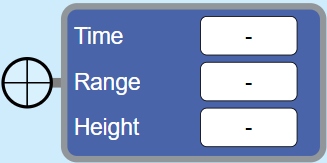
\includegraphics[width=4cm]{physics/figures/phet-projectile-motion.png}}} node[above=1cm]{\texttt[red]{Tool \#1}};
    \end{tikzpicture}
    \hspace{5mm}
    \begin{tikzpicture}
        \begin{scope}
            \clip (0,-0.03) circle (0.87);
            \draw (0,0) node {\fbox{
\includegraphics[width=2cm]{physics/figures/phet-projectile-motion-3.png}}};
            \draw[thick] (0,-0.03) circle (0.85);
        \end{scope}
        \node[above=8mm] at (0,0) {\texttt[red]{Reset button}};
    \end{tikzpicture}
\end{center}

The \texttt[red]{Tool \#1} measures time, range, and height at several points on the path of a projectile. \texttt[red]{Time} is the time elapsed since the launch of the projectile, \texttt[red]{Range} is the projectile's horizontal displacement from the origin, and \texttt[red]{Height} is the projectile's vertical displacement from the origin. Three special points on the trajectory are worth mentioning. First, the origin, which is where the cannon is positioned, defines the initial horizontal and vertical positions of the projectile as zero: $x_0=0$ and $y_0 = 0$. Second, the maximum height occurs when the reaches its largest vertical displacement, and, third, maximum range occurs when the projectile impacts the ground. 

\begin{center}
    \begin{tikzpicture}[
        declare function={f(\x,\yi,\vi,\thetai)=\yi + tan(\thetai)*\x - \grav*\x^2/(2*(\vi*cos(\thetai))^2);}, %equation of path
        declare function={R(\vi,\thetai) = \vi^2 * sin(2*\thetai) / \grav;}, % maximum range
        declare function={h(\vi,\thetai) = (\vi*sin(\thetai))^2/(2*\grav);} %maximum height
    ]
    \tikzmath{
        \grav=9.8;
    }
    \pgfplotsset{compat=1.11}
        \begin{axis}[width=7cm,height=7cm,ticks=none,
        axis lines = center,
        axis line style={draw=none},
        clip=false,
        xmin=0, xmax={R(18,80)*1.1},
        ymin=0, ymax={h(18,80)*1.1},
        ]
        \draw[thick,blue,domain=0:{R(18,80)},variable=\x,samples=200] plot ({\x},{f(\x,0,18,80)});
        \node[left] at (0,0) {origin};
        \node[rotate=72,blue] at (2,7) {trajectory};
        \draw (0.6,0) arc (0:35:2) node[pos=0.8,right=2pt] {\ang{80}};
        \draw[<->,dashed] (0,0) -- ++(axis direction cs: {R(18,80)},0) node[pos=0.8,below] {maximum range};
        \draw[<->,dashed] ({R(18,80)/2},0) -- ++(axis direction cs: 0,{h(18,80)}) node[above] {maximum height};
        \end{axis}
    \end{tikzpicture}
\end{center}

\vspace{1em}

\textbf{Part I: Measuring Time, Range, and Height}

\begin{enumerate}
    \item Click the \texttt[red]{Fire} button to launch a cannonball from the cannon. Observe that the path of the projectile is indicated by the blue curve. A projectile's path is called the trajectory.
    \item Draw a sketch of the trajectory. 
    \item \label{VSHLLm} Use \texttt[red]{Tool \#1} to measure time, range, and height data throughout the trajectory at 0.4-second time intervals. In other words, at times $t=\SI{0.0}{s}$, \SI{0.4}{s}, \SI{0.8}{s}, \ldots, \SI{3.6}{s}. Label your data on the sketch from Step \ref{VSHLLm}.
    \item Record time, range, and height at these three points: the origin, at maximum height, and at maximum range.
\end{enumerate}



\vspace{1em}

\textbf{Part II: How Mass Affects Projectile Path}

\begin{enumerate}
    \item The \texttt[red]{Reset} button ($\boldsymbol{\circlearrowleft}$) is located at the bottom right corner. It resets all settings to the default, as you found the page when you first opened it. Click the $\boldsymbol{\circlearrowleft}$ button.
    \item Click the \texttt[red]{Fire} button to launch a cannonball. Observe the same path, or the so-called trajectory, as before.
    \item \label{thVv3G} The default mass of the cannonball is \SI{17.60}{kg}. Change the mass to \SI{3.00}{kg}, and fire the cannon again. Did the trajectory change? Record your observations. 
    \item Repeat Step \ref{thVv3G} using the following projectile masses: $m=\SI{10}{kg}$, \SI{25}{kg}, and \SI{31}{kg}. Record your observations for each case. Then answer the following question: How does changing the mass of a projectile affect its path?
\end{enumerate}

\vspace{1em}

\textbf{Part III: How Launch Height Affects Projectile Path}
\begin{enumerate}
    \item Click the \texttt[red]{Reset} ($\boldsymbol{\circlearrowleft}$) button.
    \item Click the \texttt[red]{Fire} button, noting the familiar trajectory in blue.
    \item Locate the cannon, at the origin. The values \SI{0}{m} and \ang{80} next to the cannon indicate that the projectile is set to be launched from a height of zero meters and at angle of \ang{80} from the horizontal.
    \item Locate the $\boldsymbol{+}$ symbol on the center of the cannon. Clicking and dragging this symbol upwards increases the launch height of the projectile. Change the launch height to 3 meters, fire the projectile at this height, and observe the new projectile path. Record your observations.
    \item Click-and-drag the $\boldsymbol{+}$ to change the launch height from 0 to 15 meters in increments of 3. In other words, from launch heights of \SI{0}{m}, \SI{3}{m}, \SI{6}{m}, \ldots, \SI{15}{m}. At each launch height, \texttt[red]{Fire} the projectile to observe the new trajectory. Record all your observations. 
    \item How does changing the launch height affect the path of a projectile? You may draw several sketches and use time, range, and height data from \texttt[red]{Tool \#1} to support your answer.
\end{enumerate}

\vspace{1em}

\textbf{Part IV: How Launch Velocity Changes Projectile Path}

\begin{enumerate}
    \item Click $\boldsymbol{\circlearrowleft}$ to reset all settings.
    \item \texttt[red]{Fire} the projectile at the default settings and observe the now-familiar trajectory. 
    \item By default, the cannon is set to fire the projectile with an initial speed (or velocity) of 18 meters per second. Decrease the velocity to \SI{12}{m/s}, \texttt[red]{Fire} the projectile, and observe the new projectile path.
    \item Increase the speed to \SI{24}{m/s}, \texttt[red]{Fire} the projectile, and observe the new trajectory.
    \item What initial speed causes the projectile to land closest to the bullseye (all other factors being equal)?
    \item How does changing launch velocity affect the path of a projectile? Draw sketches and reference time, range, and height data from \texttt[red]{Tool \#1} to support your answer.
\end{enumerate}





    

\end{document}